%
%	Begrifflichkeiten
%

\pagebreak
\section{Targeting}

\onehalfspacing

\subsection{Targeted Advertising}

\subsubsection{Rationale}

"Microtargeting is a marketing strategy that uses people’s data — about what they like, who they’re connected to, what their demographics are, what they’ve purchased, and more — to segment them into small groups for content targeting. It’s the reason that if you typically shop at Whole Foods, you may be served an advertisement for organic sunscreen during the Summer. And while it can help deliver content that is interesting and helpful to you, it also has a dark side — especially if it delivers information that’s inaccurate or biased and meant to sway your vote."\footnote{\textit{Ghosh, D. (2018)}: What is microtargeting? \cite{mozillaBlog}}

To be written.

\subsubsection{Tracking}

Tracking is under attack from multiple angles\footnote{See \textit{Brinkmann, M. (2021)}: How Firefox new SmartBlock feature works \cite{mozillaBlog}}

To be written.

\subsubsection{Cookies}

We will focus on Cookies and web browser as the main tracking mechanisms.

There's also tracking in E-Mail\footnote{See \textit{Doffmann, Z. (2021)}: Why You Suddenly Need To Delete Gmail On Your iPhone \cite{deleteGmail}}, which we will ignore for this paper.

To be written.

\subsection{Data Types}

\subsubsection{First-Party Data}

To be written.

\subsubsection{Second-Party Data}

To be written.

\subsubsection{Third-Party Data}

To be written.

\subsection{Toolstacks}

\subsubsection{Google Analytics}

To be written.

\begin{figure}[H]
\centering
\caption {Plausible}
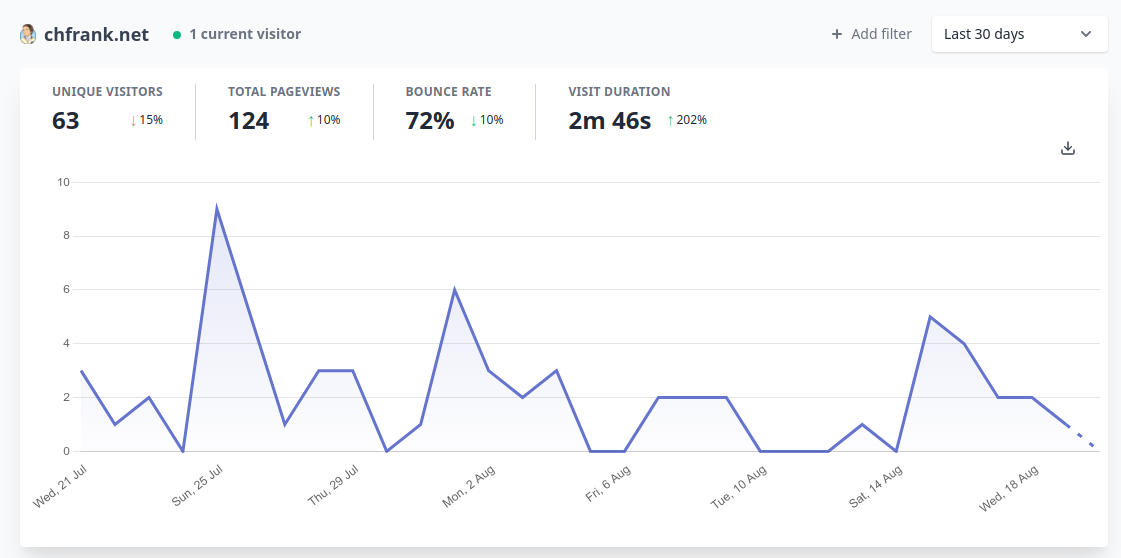
\includegraphics[width=\linewidth]{images/plausible.png}
\label{fig:plausible}
\end{figure}

\subsubsection{Google Ads}

To be written.

\subsubsection{Amazon Advertising}

To be written.

\subsubsection{Facebook Advertising}

To be written.

\subsubsection{Yandex Metrica}

To be written.

\subsection{Moving past cookies}

\subsubsection{Browser-based}

\paragraph{Google FLoC}

To be written

\paragraph{}{Microsoft Parakeet}

To be written.

\subsubsection{First Party Data-based}

\paragraph{Data Clean Rooms}

To be written.

\subsubsection{Identity-based}

\paragraph{UID2}

To be written.

\paragraph{Apple Identifier for Advertisers (IDFA)}

To be written.

\paragraph{Android Advertising ID (AAID) / Google Advertising ID (GAID)}

To be written.

\subsubsection{Content-based targeting}

To be written.

\subsection{Legal Framework}

\subsubsection{GDPR (General Data Protection Regulation) / UK-GDPR}

To be written.

\subsubsection{DS-GVO (Datenschutz-Grundverordnung)}

To be written.

\subsubsection{EU e-Privacy Proposal}

To be written.

\subsubsection{Telekommunikations-Telemedien-Datenschutz-Gesetz (Entwurf)}

To be written.

\subsubsection{Other Legal Frameworks}

\begin{itemize}
 \item CCPA (California Consumer Privacy Act)
 \item LGPD (Lei Geral de Proteção de Dados Pessoais)
 \item POPIA (Protection of Personal Information Act)
 \item DSA (Digital Services Act)
 \item DMA (Digital Markets Act)
\end{itemize}


